%%%%%%%%%%%%%%%%%%%%%%%%%%%%% Define Article %%%%%%%%%%%%%%%%%%%%%%%%%%%%%%%%%%
\documentclass{article}
%%%%%%%%%%%%%%%%%%%%%%%%%%%%%%%%%%%%%%%%%%%%%%%%%%%%%%%%%%%%%%%%%%%%%%%%%%%%%%%

%%%%%%%%%%%%%%%%%%%%%%%%%%%%% Using Packages %%%%%%%%%%%%%%%%%%%%%%%%%%%%%%%%%%
\usepackage{geometry}
\usepackage{graphicx}
\usepackage{amssymb}
\usepackage{amsmath}
\usepackage{amsthm}
\usepackage{empheq}
\usepackage{mdframed}
\usepackage{booktabs}
\usepackage{lipsum}
\usepackage{graphicx}
\usepackage{color}
\usepackage{psfrag}
\usepackage{pgfplots}
\usepackage{bm}
\usepackage[colorlinks=true, urlcolor=blue, linkcolor=red]{hyperref}
%%%%%%%%%%%%%%%%%%%%%%%%%%%%%%%%%%%%%%%%%%%%%%%%%%%%%%%%%%%%%%%%%%%%%%%%%%%%%%%

% Other Settings

%%%%%%%%%%%%%%%%%%%%%%%%%% Page Setting %%%%%%%%%%%%%%%%%%%%%%%%%%%%%%%%%%%%%%%
\geometry{a4paper}

%%%%%%%%%%%%%%%%%%%%%%%%%% Define some useful colors %%%%%%%%%%%%%%%%%%%%%%%%%%
\definecolor{ocre}{RGB}{243,102,25}
\definecolor{mygray}{RGB}{243,243,244}
\definecolor{deepGreen}{RGB}{26,111,0}
\definecolor{shallowGreen}{RGB}{235,255,255}
\definecolor{deepBlue}{RGB}{61,124,222}
\definecolor{shallowBlue}{RGB}{235,249,255}
%%%%%%%%%%%%%%%%%%%%%%%%%%%%%%%%%%%%%%%%%%%%%%%%%%%%%%%%%%%%%%%%%%%%%%%%%%%%%%%

%%%%%%%%%%%%%%%%%%%%%%%%%% Define an orangebox command %%%%%%%%%%%%%%%%%%%%%%%%
\newcommand\orangebox[1]{\fcolorbox{ocre}{mygray}{\hspace{1em}#1\hspace{1em}}}
%%%%%%%%%%%%%%%%%%%%%%%%%%%%%%%%%%%%%%%%%%%%%%%%%%%%%%%%%%%%%%%%%%%%%%%%%%%%%%%

%%%%%%%%%%%%%%%%%%%%%%%%%%%% English Environments %%%%%%%%%%%%%%%%%%%%%%%%%%%%%
\newtheoremstyle{mytheoremstyle}{3pt}{3pt}{\normalfont}{0cm}{\rmfamily\bfseries}{}{1em}{{\color{black}\thmname{#1}~\thmnumber{#2}}\thmnote{\,--\,#3}}
\newtheoremstyle{myproblemstyle}{3pt}{3pt}{\normalfont}{0cm}{\rmfamily\bfseries}{}{1em}{{\color{black}\thmname{#1}~\thmnumber{#2}}\thmnote{\,--\,#3}}
\theoremstyle{mytheoremstyle}
\newmdtheoremenv[linewidth=1pt,backgroundcolor=shallowGreen,linecolor=deepGreen,leftmargin=0pt,innerleftmargin=20pt,innerrightmargin=20pt,]{theorem}{Theorem}[section]
\theoremstyle{mytheoremstyle}
\newmdtheoremenv[linewidth=1pt,backgroundcolor=shallowBlue,linecolor=deepBlue,leftmargin=0pt,innerleftmargin=20pt,innerrightmargin=20pt,]{definition}{Definition}[section]
\theoremstyle{myproblemstyle}
\newmdtheoremenv[linecolor=black,leftmargin=0pt,innerleftmargin=10pt,innerrightmargin=10pt,]{problem}{Problem}[section]
%%%%%%%%%%%%%%%%%%%%%%%%%%%%%%%%%%%%%%%%%%%%%%%%%%%%%%%%%%%%%%%%%%%%%%%%%%%%%%%

%%%%%%%%%%%%%%%%%%%%%%%%%%%%%%% Plotting Settings %%%%%%%%%%%%%%%%%%%%%%%%%%%%%
\usepgfplotslibrary{colorbrewer}
\pgfplotsset{width=8cm,compat=1.9}
%%%%%%%%%%%%%%%%%%%%%%%%%%%%%%%%%%%%%%%%%%%%%%%%%%%%%%%%%%%%%%%%%%%%%%%%%%%%%%%

%%%%%%%%%%%%%%%%%%%%%%%%%%%%%%% Title & Author %%%%%%%%%%%%%%%%%%%%%%%%%%%%%%%%
\title{Method of Moving Points}
\author{Alston Yam}
\date{}
\parskip=5pt
\parindent=0pt
%%%%%%%%%%%%%%%%%%%%%%%%%%%%%%%%%%%%%%%%%%%%%%%%%%%%%%%%%%%%%%%%%%%%%%%%%%%%%%%

\begin{document}
    \maketitle

    \section{Introduction}
    Inspired by \href{https://web.evanchen.cc/static/mop/mockimo/2020.pdf}{problem 4} on this IMO mock by Evan Chen.

    \section{Cross Ratios}
    \begin{definition}[Cross Ratios]
        Given 4 distinct points $A, B, C, D$ on a line, the cross ratio $(A, B; C, D)$ is defined as \[(A, B; C, D) = \frac{AC \cdot BD}{BC \cdot AD}\]
        Where the lengths are taken to be directed $(XY = -YX)$.
    \end{definition}

    We can actually extend the definition of the cross ratio to not just points on a line, but also four points on a conic $\gamma$ (the most commonly used conic in Olympiad geometry is a circle), and also a \textit{pencil} of lines through a particular point. In the latter case $A, B, C, D$ will correspond to lines rather than points.

    In the case of a pencil, the cross ratio can actually be thought of as the ratio of the sines of the angles between these four lines. 

    \section{Projective Transformations}

    A \textit{projective transformation} is any transformation that preserves the cross ratio. Specifically:

    \begin{definition}[Projective Transformations]
        A projective map $f$ is defined as a function $f:\mathcal{C}_1 \to \mathcal{C}_2$ (where $\mathcal{C}_1$ and $\mathcal{C}_2$ are both conics, lines or pencils of lines) such that for any 4 points $A, B, C, D \in \mathcal{C}_1$, \[(A, B; C, D) = (f(A), f(B); f(C), f(D))\]
    \end{definition}

    Notice that a projective map is bijective. Now, here are two results that would come in handy.

    \begin{theorem}[Projective Compositions]
        The composition $f \circ g$ of two projective functions $f$ and $g$ is projective.
    \end{theorem}

    \begin{proof}
        \[(A, B; C, D) = (g(A), g(B); g(C), g(D)) = (f \circ g(A), f \circ g(B); f \circ g(C), f \circ g(D))\]
    \end{proof}

    \begin{theorem}[Inverse of a Projective Map]
        The inverse $f^{-1}$ of a projective map $f$ is also projective.
    \end{theorem}

    \begin{proof}
        \[(f(A), f(B); f(C), f(D)) = (A, B; C, D) = (f^{-1}f(A), f^{-1}f(B); f^{-1}f(C), f^{-1}f(D))\]
    \end{proof}

    

    We give a few examples of common projective transformations below. These are taken from \href{https://artofproblemsolving.com/community/c473124h1763266_moving_points_tutorial}{this blog post}.


    \subsection{Common Projective Transformations}
    \subsubsection{Projection from a line to a pencil of lines}
    Given a line $l$ and a point $P$ not on $l$, we can project every point $Q$ on $l$ to the line $PQ$. This is a projective map, as \[(A, B; C, D) = (PA, PB; PC, PD)\] Where $PA, PB, PC, PD$ are lines going through $P$.  

    \subsubsection{Projection from a line to another line}
    To project a line $l_1$ to another line $l_2$, we take a point $P$ not on either line. We will first project $l_1$ onto the pencil of lines going through $P$, then project this pencil onto $l_2$. This gives the desired effect.

    \subsubsection{Rotating a pencil of lines}
    This is a projective map as the cross ratio of a pencil of lines only depend on the angle between them.

    \subsubsection{Reflection across a line}
    This is true by symmetry: imagine four points $A, B, C, D$. When we reflect them across any arbitrary line $l$, The distances between them (in the case they are points) or the angle between them (in in case they are lines) stays fixed.

    \subsubsection{Projection from a conic to a pencil of lines}

    Consider a conic $\gamma$. We take a point $P \in \gamma$, and for every other point $Q \in \gamma, Q \not= P$, we will project $Q$ onto the line $PQ$. 

    \subsubsection{Projection from a conic to points on that same conic}
    Consider the conic $\gamma$ once again. Now we will take a point $P$ not on the conic. For every point $Q$ on the conic, we will project $Q$ to $PQ \cap \gamma$ different from $Q$ (Unless $PQ$ is a tangent, in which case $Q$ gets mapped to itself).

    \subsubsection{Inversion}
    It turns out, interestingly, Inversion also preserves the cross ratio. Therefore inversion is actually also a type of projective transformation.
    \begin{proof}
        Consider an inversion about a circle with radius $r$ and center $O$. By the distance formula: \[A'B' = \frac{r^2}{OA \cdot OB} \cdot AB\]
        Now we have: 
        \[(A', B'; C', D') = \frac{A'C' \cdot B'D'}{B'C' \cdot A'D'} = \frac{\frac{r^4}{OA \cdot OB \cdot OC \cdot OD} \cdot AC \cdot BD}{\frac{r^4}{OA \cdot OB \cdot OC \cdot OD} \cdot BC \cdot AD} = \frac{AC \cdot BD}{BC \cdot AD} = (A, B; C, D)\]
    \end{proof}

    \section{The Method}
    The essence of the method of moving points boils down to one important theorem:
    \begin{theorem}
        If $f, g: \mathcal{C}_1 \to \mathcal{C}_2$ are projective, then $f \equiv g$ iff $f(A)=g(A)$ for at least 3 different values of A. 
    \end{theorem}

    \begin{proof}
        Necessity is simple. Now for sufficiency: consider 3 points $A, B, C$ such that $f=g$ on these three points. Consider another point $X \in \mathcal{C}_1/_{\{A, B, C\}}$ Then we see: 
        \[(f(A), f(b); f(C), f(X)) = (A, B; C, X) = (g(A), g(B); g(C), g(X)) = (f(A), f(b); f(C), g(X))\]
        Which is enough to conclude $f(X) = g(X)$. 
    \end{proof}

    So now to solve a given geometry problem, If we can find two projective maps $f$ and $g$, such that $f$ is equivalent to the condition given by the problem, and $g$ is equivalent to the result we want to prove, then we only need to check 3 special values of a moving point where $f=g$. If we can do that, then by the above theorem we would've proved that $f \equiv g$ and in fact we would be done.

    \section{Example Problem}
    Sourced from \href{https://artofproblemsolving.com/community/c473124h1763266_moving_points_tutorial}{this blog}.

    \begin{problem}[USA Winter TST for IMO 2019 Problem 1]
        Let $ABC$ be a triangle and let $M$ and $N$ denote the midpoints of $\overline{AB}$ and $\overline{AC}$, respectively. Let $X$ be a point such that $\overline{AX}$ is tangent to the circumcircle of triangle $ABC$. Denote by $\omega_B$ the circle through $M$ and $B$ tangent to $\overline{MX}$, and by $\omega_C$ the circle through $N$ and $C$ tangent to $\overline{NX}$. Show that $\omega_B$ and $\omega_C$ intersect on line $BC$. \\\\
        \textit{Merlijn Staps}
    \end{problem}

    \begin{center}
        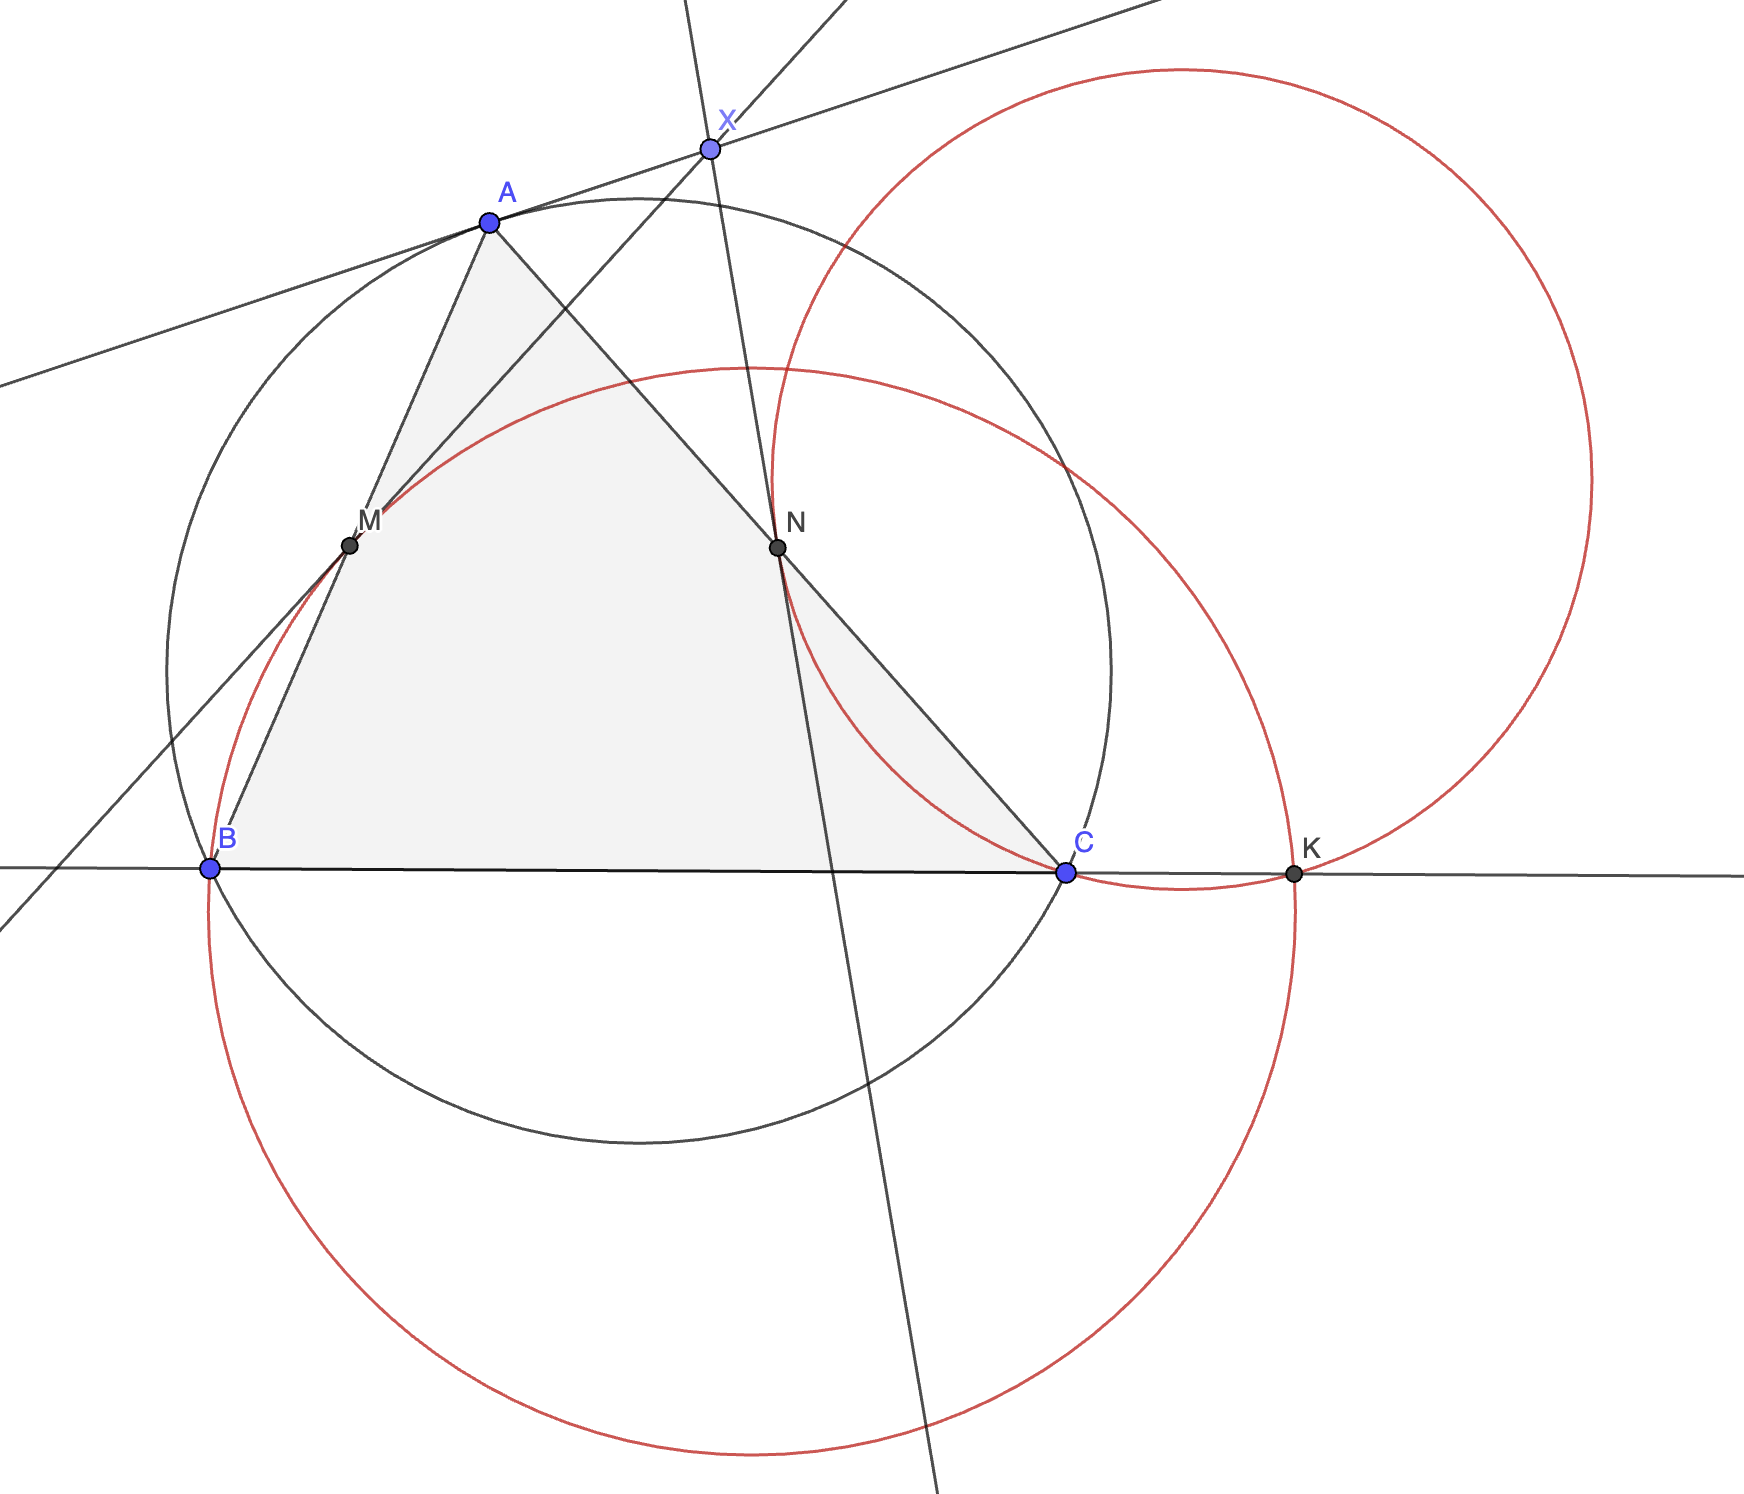
\includegraphics[scale=0.3]{Diagram.png}
    \end{center}
    
    \begin{proof}
        Call the tangent at $A$ $l_1$, and call line $BC$ $l_2$. 
        
        We will define a map $f:l_1 \to l_2$ such that $f(X) = K$. Specifically, see that $f$ can be thought of as 3 projections: $l_1$ will be projected to the pencil of lines at $N$, then we rotate this pencil at $N$ by $\angle NCK$. We finally project this rotated pencil onto $(NKC)$ which coincides with $l_2$ at $K$ (This works via the tangent property).

        Similarly, lets define another projection $g$ that does the same thing to the other side. Now we have two projective functions $f$ and $g$, so it suffices to check three particular cases to prove that $f\equiv g$.

        \textcolor{red}{Case 1:} $X$ = $A$. Then we see $f(X) = P_{\infty}$, and similarly $g(X) = P_{\infty}$, so $f(X) = g(X)$ here.
        
        \textcolor{red}{Case 2:} Pick $X$ such that $\angle XNC$ = $180 - \angle ACB$. We see that in this case, $f(X) = C$. Now we aim to show that $g(X) = C$ too. I will now prove $\angle XMC = \angle ABC$, which would imply the result. Notice that $\triangle ANX \sim \triangle MNA$ via an angle chase. Hence, $\frac{XA}{AN} = \frac{AM}{MN} \iff \frac{AM}{XA} = \frac{MN}{AN} = \frac{MN}{NC}$. Also $\angle MNC$ = $\angle MAX$, so $\triangle MAX \sim \triangle MNC$. Now we have $\angle XMC = \angle NMA = \angle ABC$, so we have $g(X) = C$ too.

        \textcolor{red}{Case 3:} Pick $X$ to be the corresponding point to Case 2, but on the other side. By the similar argument we have $f(X) = g(X) = B$, so we're done.

        Now we have found 3 points, we may conclude that $f\equiv g$ and so we're done.
    \end{proof}

    
\end{document}